% !TeX encoding=unicode
% !TeX spellcheck = en-US

\chapter{Results}
%
\section{Study of the Higgs transverse momentum}
\ldots

Four seperate runs have been performed: One run each for zero, one and two jets at fixed order NLO and one \mcatnlo{} run merging up to two jets in the core process.
The \rivet{} analysis system has been used to extract the transverse momentum of the Higgs boson from the events.
In the multijet merged run, the cases of at least zero, one or two jets have been distinguished and sorted into different histograms.
Thus, we obtain inclusive observables that are comparable to the fixed order results.
\sherpa{} has been used for all calculations and the \mcfm{} library \cite{mcfm_hjj} has been interfaced for the 2-jet process.
For the fixed order calculations, both the renormalization and the factorization scale have been set to the transverse mass of the Higgs boson.
Final state jets have been extracted by the \fastjet{} library \cite{fastjet_manual} using the anti-$k_t$ algorithm \cite{anti_kt} with a radius parameter $R=0.4$ and a $p_\perp$-cut of $p_\perp > \SI{20}{\giga\electronvolt}$.

\Cref{fig:h_hpt_nominal} compares the fixed order NLO and the merged \mcatnlo{} results in the case of no jets.
At NLO the tranverse momentum of the Higgs boson arises solely from real gluon emissions as the LO process does not have any tranverse parts.
The splitting leading to the real emissions is divergent in the soft and collinear limits which correspond to low transverse momenta.
Therefore, in \cref{fig:h_hpt_nominal}, we see that the cross section diverges towards low $p_\perp$.
The multijet result behaves completely different in the low $p_\perp$ region and shows no divergence.
In this case, the cross section is dominated by parton showers which include higher orders and are not divergent.
Compared to the fixed order calculation, the cross section is much smaller in the low $p_\perp$ region.
As opposed to this, the cross section is amplified for $p_\perp \gtrsim \SI{20}{\giga\electronvolt}$.
The influence of the parton shower is neglible in this region.
Instead the additional contributions come from the higher jet multiplicities that have been merged into the calculation.
At high $p_\perp$, both results approach each other.

The results containing one or more jets are compared in \cref{fig:hj_hpt_nominal}.
The total cross section expectably is smaller than in the 0-jet case.
Due to the jet cut, the minimum $p_\perp$ of the Higgs boson is \SI{20}{\giga\electronvolt}.
At $p_\perp = \SI{20}{\giga\electronvolt}$, when the Higgs boson recoils against the jet, the cross section diverges at NLO.
Similar to the previous situation, the parton shower fixes the divergence and produces a smooth distribution.
At high $p_\perp$ the merged run gives a higher cross section, this time the additional contributions stem from the 2-jet process.
%
\begin{figure}
	\centering
	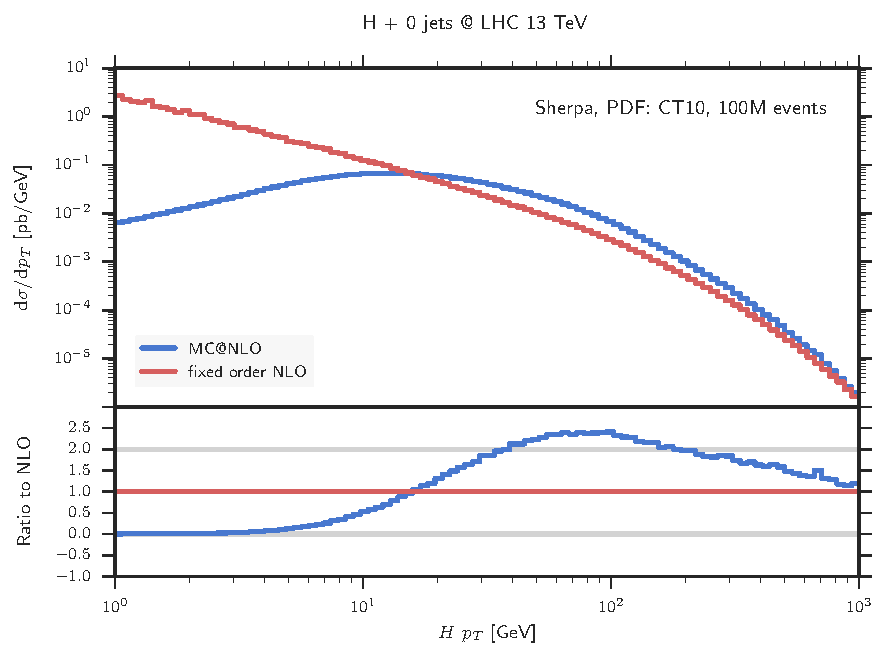
\includegraphics[width=0.8\textwidth]{images/h_hpt_nominal.pdf}
	\caption{H pT 0j}
	\label{fig:h_hpt_nominal}
\end{figure}
%
\begin{figure}
	\centering
	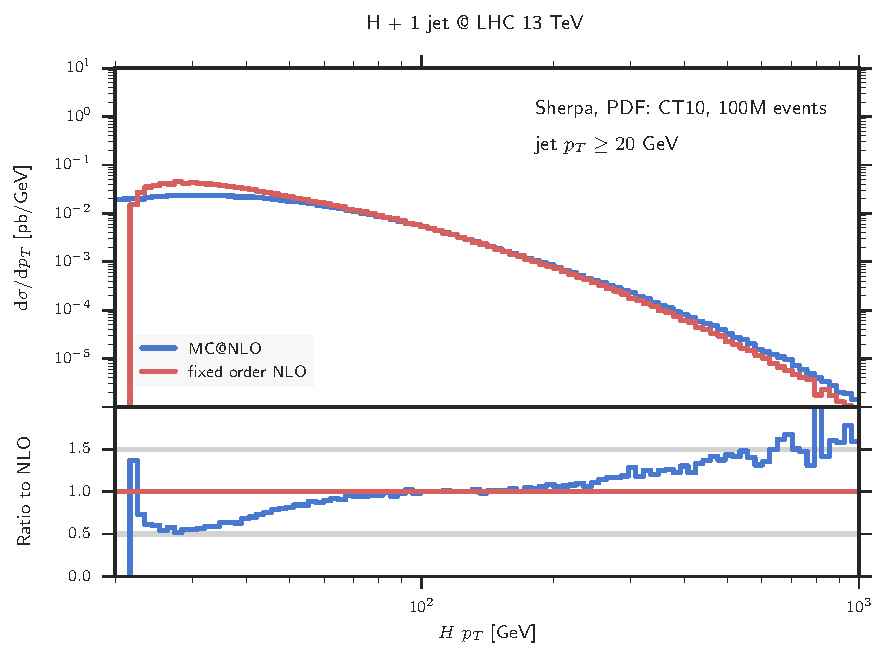
\includegraphics[width=0.8\textwidth]{images/hj_hpt_nominal.pdf}
	\caption{H pT 1j}
	\label{fig:hj_hpt_nominal}
\end{figure}
%
\begin{figure}
	\centering
	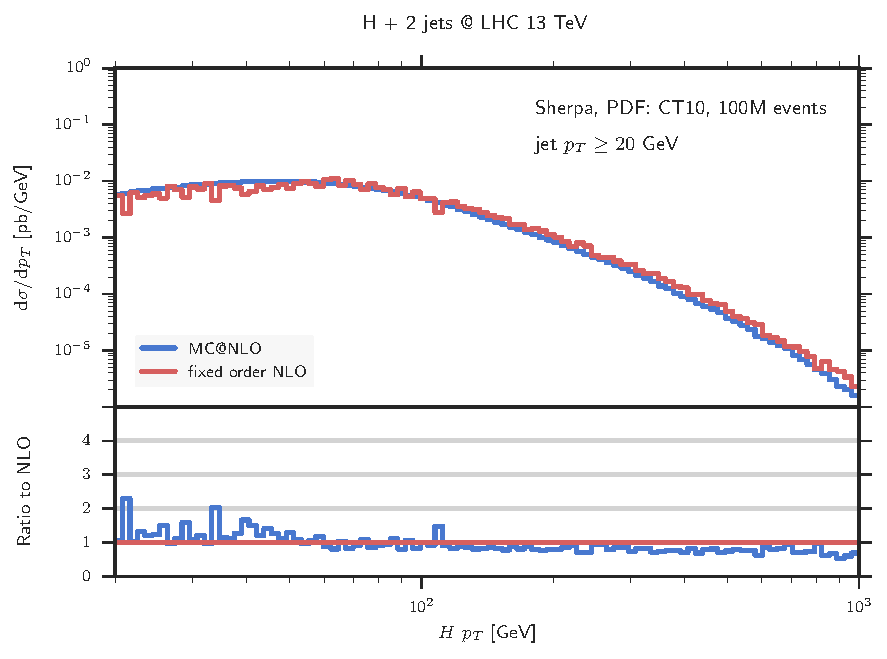
\includegraphics[width=0.8\textwidth]{images/hjj_hpt_nominal.pdf}
	\caption{H pT 2j}
	\label{fig:hjj_hpt_nominal}
\end{figure}
%
\section{Grid validiation}
In the following we will validate the interpolation method used by \mcgrid{} for the processes $pp \rightarrow H + (0,1,2) \text{jets}$ at the \SI{13}{\tera\electronvolt} LHC, computed at NLO.
Thereto, we generate reference distributions for different observables using the \sherpa{} event generator and compare them to the distributions obtained by convoluting a grid with the respective PDF.
Additionally, the results from \appl{} and \fnlo{} are compared to each other.
All grids are filled using the central value of the CT10 pdf set \cite{ct10}.
The examined observables are the transverse momenta $p_\perp$ of the Higgs boson and the $\tau$ leptons, respectively, the rapidity $y$ of the Higgs boson and the pseudorapidity $\eta$ of the $\tau$ leptons.
The projection of the observables into histogram bins is accomplished by the \rivet{} analysis system.
Final state jets are extracted by the \fastjet{} library \cite{fastjet_manual} using the anti-$k_t$ algorithm \cite{anti_kt} with a radius parameter $R=0.4$ and a $p_\perp$-cut of $p_\perp > \SI{20}{\giga\electronvolt}$.

The first validity test will check whether the grids are able to reproduce the distributions when they are filled with the same events as the reference histograms, i.e.\ when no parameter variation is performed.
This will also determine the interpolation accuracy.
Subsequently, the cases where the scale factors and/or PDFs of the grids are changed \textit{a posteriori} will be compared to reference distributions where these parameters have been set explicitly.
%
\subsection{Interpolation accuracy}
In this section we will prove, that the grids are able to reproduce the reference distributions up to the available interpolation accuracy.
For each observable, one high precision grid and one lower precision grid is used.
In the 0- and 1-jet cases, the high precision grid has \num{50} bins in $x$ and the lower precision grid has \num{30} bins in $x$.
In the 2-jet case, the high precision grid has \num{70} bins and the lower precision one has \num{50} bins.
This is because with higher jet multiplicity, the influence of high $x$ values increases while in all cases the same transformation is used to smooth the distribution.
As we have seen in \textcolor{red}{???????????????????????????????}, this transformation favors low values of $x$, so a relatively high number of grid points is needed to accurately represent the high $x$ region.
For all the following calculations, the scale parameters have been fixed to the mass of the Higgs boson.
Therefore, $Q^2$ does not change and only one bin is used.
To achieve better comparability, \appl{} is configured to use fourth order interpolation, which is the same as is hardcoded into the \fnlo{} library.
A sample of \num{1} million events is used to fill the grids.

\Cref{fig:hnlo_validation} shows the ratio of the results obtained by convoluting the grids with the CT10 PDF to the reference distributions for the 0-jet process.
Using the high precision grid, almost all bins show errors below \SI{0.1}{\percent}.
\appl{} and \fnlo{} show roughly the same accuracy but the lepton $p_\perp$ shows a few outliers with \fnlo{}.
The effect of using a smaller grid is considerably bigger for the $p_\perp$ distributions than for the rapidity distributions.
It is also bigger for \appl{} than for \fnlo{}.

With one jet (\cref{fig:hjnlo_validation}), the errors in the reproduction of the $p_\perp$ become notably larger, especially when using \fnlo{}.
There are comparatively large outliers using the lower precision grids.
Nonetheless, with the high precision grids the errors are still within \SI{0.3}{\percent}.

The case of two jets is shown in \cref{fig:hjjnlo_validation}.
Here the grid with \num{50} bins produces relatively large errors.
Though the plot does not comprise this, the highest errors are at the order of one percent.
However \textcolor{red}{\ldots}



%
\begin{sidewaysfigure}
\centering
\begin{subfigure}[]{0.49\textwidth}
	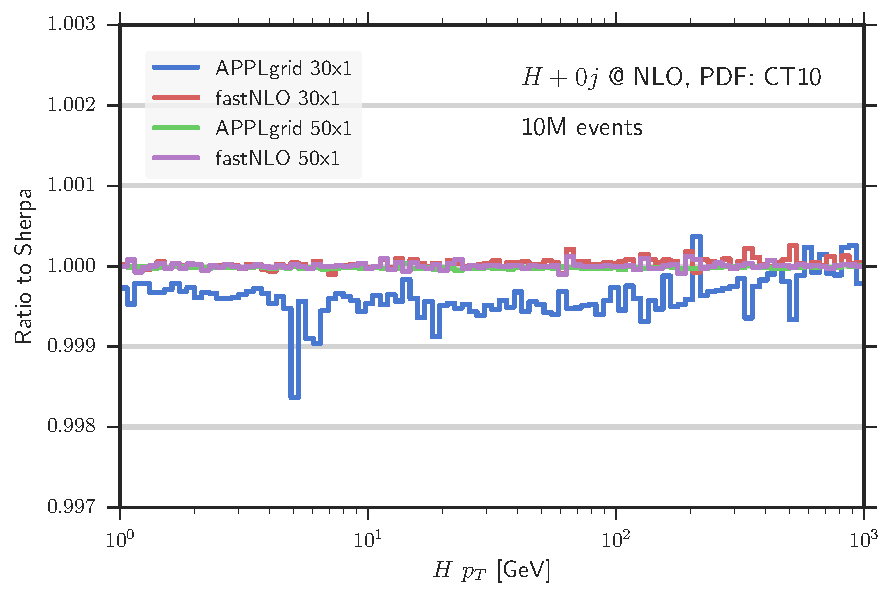
\includegraphics[width=\textwidth]{images/hnlo_hpt_50v30.pdf}
\end{subfigure}
\hfill
\begin{subfigure}[]{0.49\textwidth}
	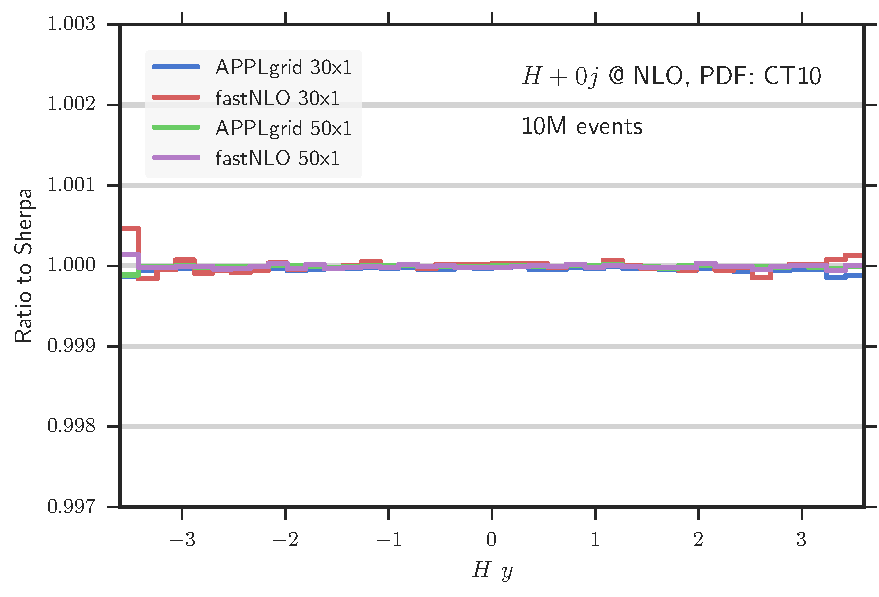
\includegraphics[width=\textwidth]{images/hnlo_hy_50v30.pdf}
\end{subfigure}

\begin{subfigure}[]{0.49\textwidth}
	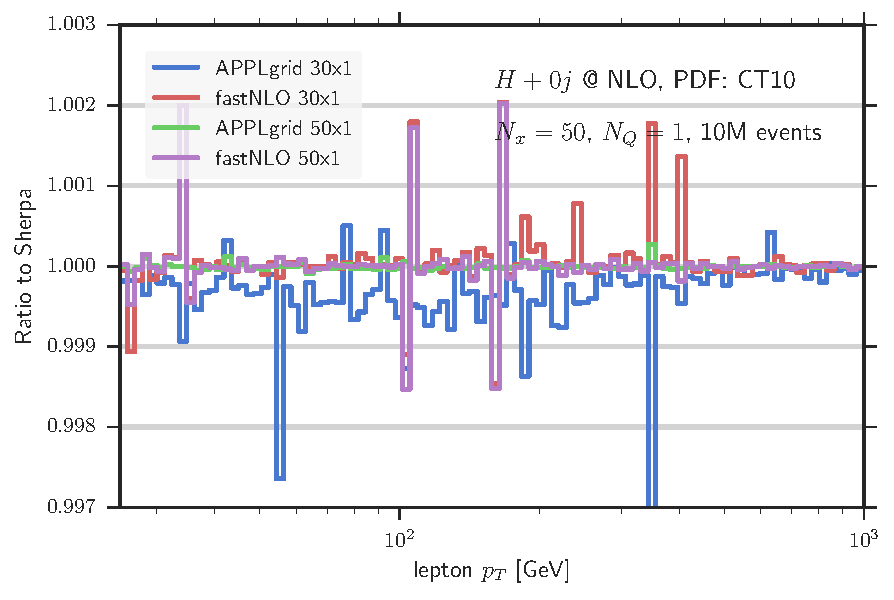
\includegraphics[width=\textwidth]{images/hnlo_lpt_50v30.pdf}
\end{subfigure}
\hfill
\begin{subfigure}[]{0.49\textwidth}
	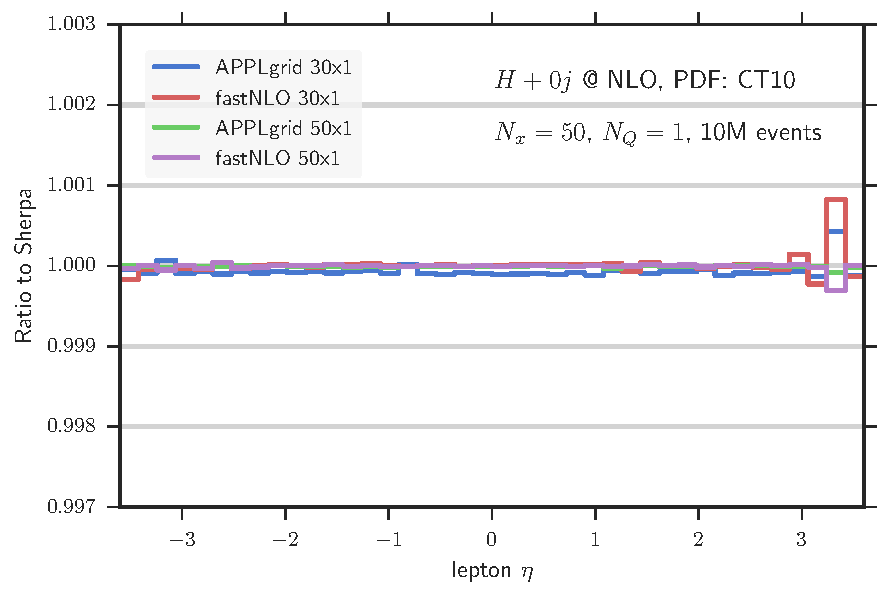
\includegraphics[width=\textwidth]{images/hnlo_leta_50v30.pdf}
\end{subfigure}
\caption{H+0j NLO}
\label{fig:hnlo_validation}
\end{sidewaysfigure}
%
\begin{sidewaysfigure}
\centering
\begin{subfigure}[]{0.49\textwidth}
	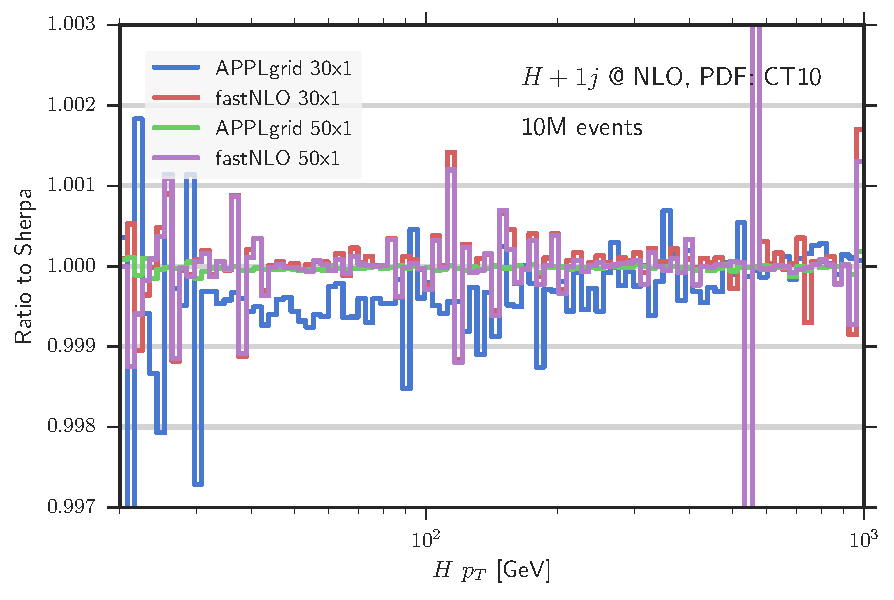
\includegraphics[width=\textwidth]{images/hjnlo_hpt_50v30.pdf}
\end{subfigure}
\hfill
\begin{subfigure}[]{0.49\textwidth}
	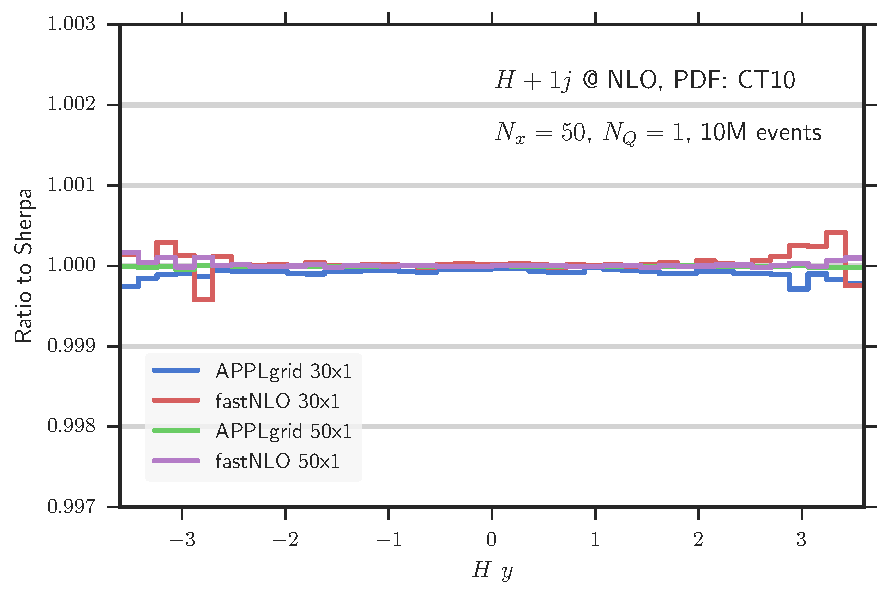
\includegraphics[width=\textwidth]{images/hjnlo_hy_50v30.pdf}
\end{subfigure}

\begin{subfigure}[]{0.49\textwidth}
	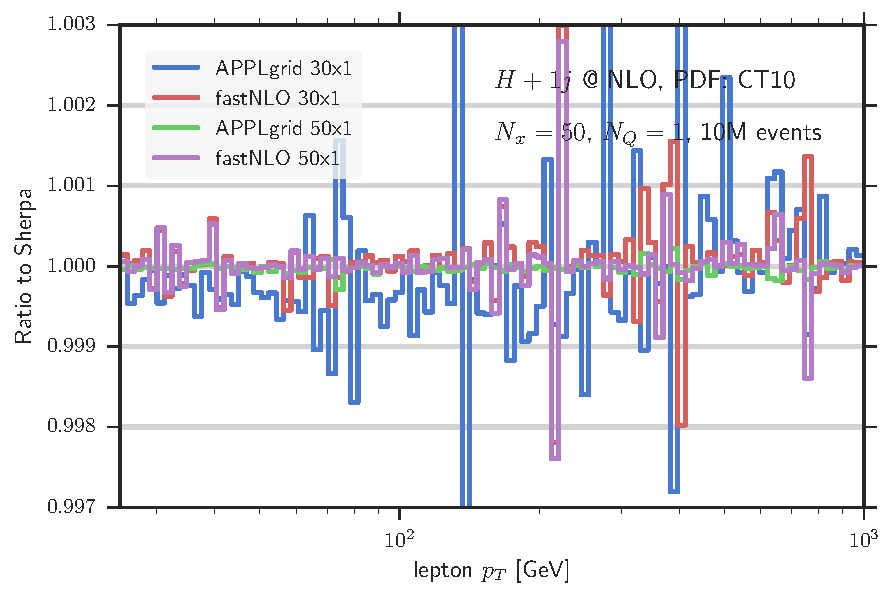
\includegraphics[width=\textwidth]{images/hjnlo_lpt_50v30.pdf}
\end{subfigure}
\hfill
\begin{subfigure}[]{0.49\textwidth}
	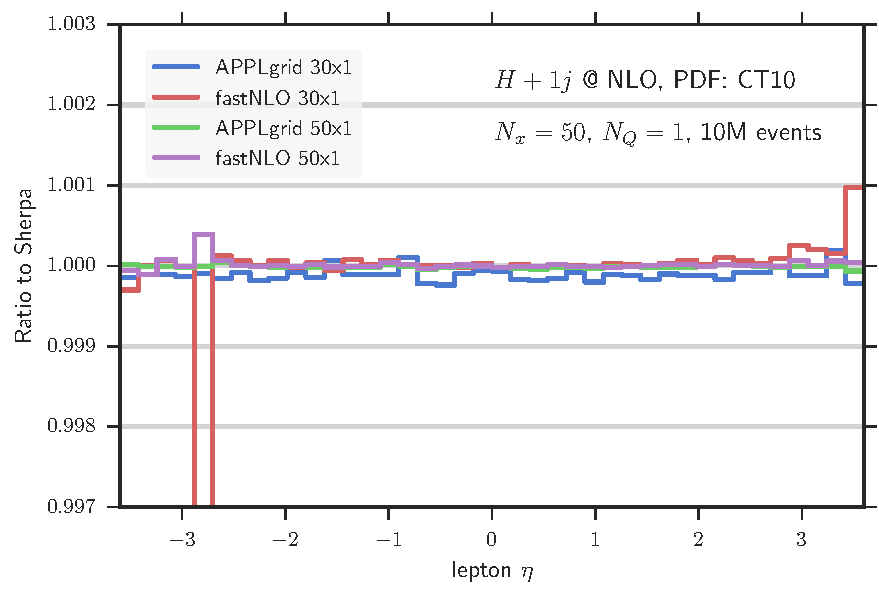
\includegraphics[width=\textwidth]{images/hjnlo_leta_50v30.pdf}
\end{subfigure}
\caption{H+1j NLO}
\label{fig:hjnlo_validation}
\end{sidewaysfigure}
%
\begin{sidewaysfigure}
\centering
\begin{subfigure}[]{0.49\textwidth}
	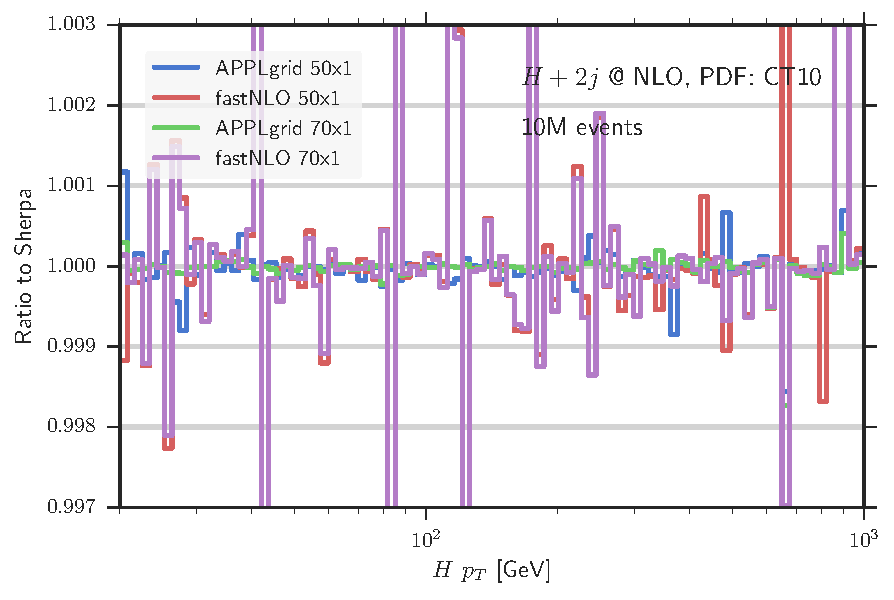
\includegraphics[width=\textwidth]{images/hjjnlo_hpt_70v50.pdf}
\end{subfigure}
\hfill
\begin{subfigure}[]{0.49\textwidth}
	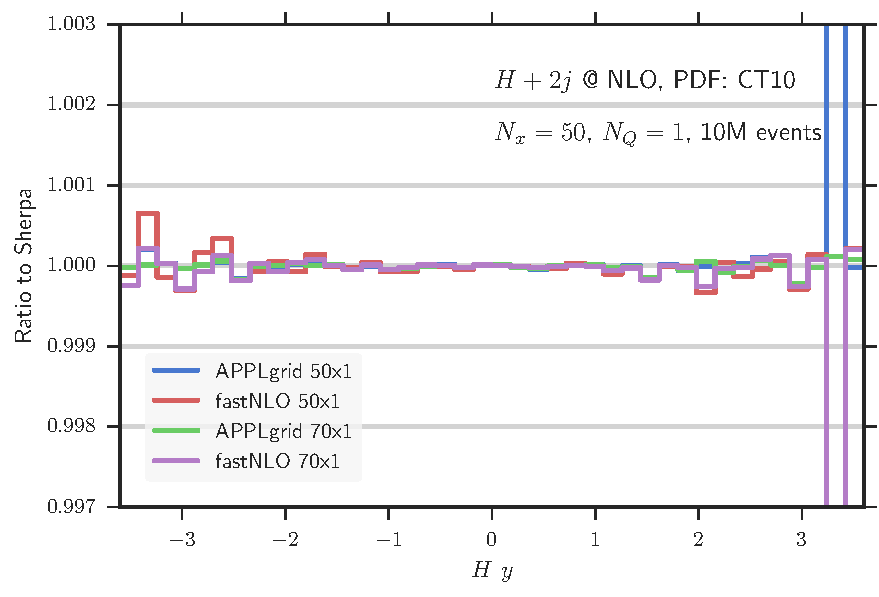
\includegraphics[width=\textwidth]{images/hjjnlo_hy_70v50.pdf}
\end{subfigure}

\begin{subfigure}[]{0.49\textwidth}
	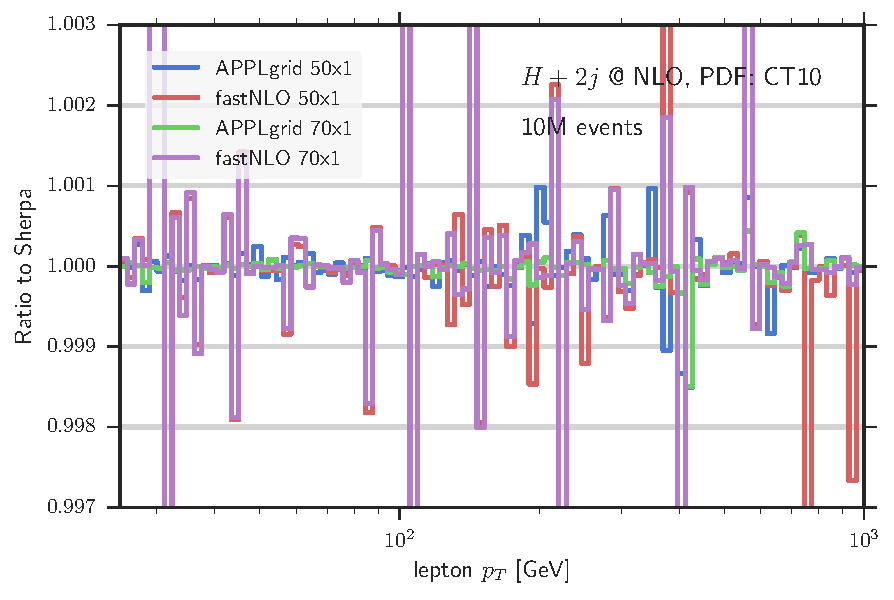
\includegraphics[width=\textwidth]{images/hjjnlo_lpt_70v50.pdf}
\end{subfigure}
\hfill
\begin{subfigure}[]{0.49\textwidth}
	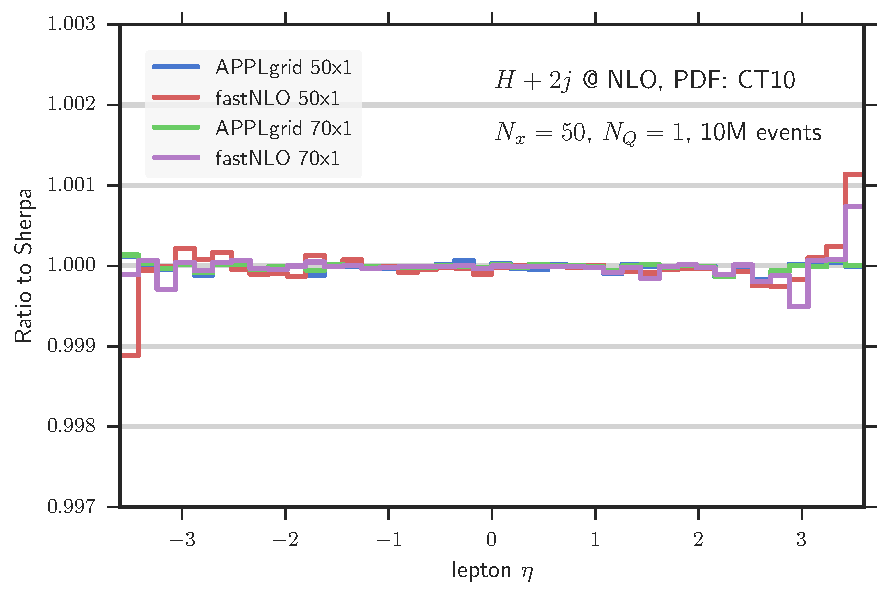
\includegraphics[width=\textwidth]{images/hjjnlo_leta_70v50.pdf}
\end{subfigure}
\caption{H+2j NLO}
\label{fig:hjjnlo_validation}
\end{sidewaysfigure}
%




\section{Scale factor variation}
Now that we have verified that the grids produced by \appl{} and \fnlo{} are able to reproduce the reference distributions up to the interpoation accuracy, we can take a look at the variation of the QCD parameters.
In this section we will examine the results obtained by varying the renormalization and factorization scales.
\appl{} and \fnlo{} both have methods implemented that allow to change the scales when calculating NLO cross sections.
There are different approaches to this.
The original method used by \appl{} is to apply the renormalization group equation for the renormalization scale and calculate the LO DGLAP splitting functions using \hoppet{} \cite{hoppet} to vary the factorization scale.
\fnlo{} originally did not allow the use of \hoppet{} and instead stored individual grids for each desired factorization scale.
This approach is not as flexible and leads to larger grid files but the calculation of the cross section is much faster.
However, since version 2.3 \fnlo{} can also be used in combination with \hoppet{}.
Another method, called \enquote{flexible-scale table}, is also implemented in \fnlo{}.
It stores fully scale-independent weights and allows for arbitrary and independent variation of the scale factors without the need of splitting functions.
As this feature is not yet implemented in \mcgrid{} (but will be in a future release), the first method is used in the following calculations.

The reference histograms are again gnerated with Sherpa using the CT10 pdf.
One central scale $\mu_R = \mu_F = m_H$ and two additional scales $2 \mu$ and $\frac{1}{2} \mu$ are used.
During the central scale run, grids for the transverse momentum of the Higgs boson are filled by \appl{} and \fnlo{} using an \mcgrid{}-enabled \rivet{} analysis.
This is done for Higgs production with zero and one jets using an event sample of 100 million events in each case.
In \cref{fig:scalesvar_hnlo_appl,fig:scalesvar_hnlo_fnlo} the reference distributions are compared to the results from \appl{} and \fnlo{} in the 0-jet case.
It can be seen that the accuracy is very good in both cases.
The discrepancies at low $p_\perp$ in \cref{fig:scalesvar_hnlo_appl} are due to an insufficient phasespace run, meaning that during the fill run $x$-values emerged that were not expected by \appl{}.
The \fnlo{} grid was prepared with the same phasespace run and obviously it responds to these events in a different way resulting in a precise reproduction throughout the range of considered values.
Using a larger phasespace run, the inaccuracies with \appl{} would of course vanish.
%
\begin{figure}
	\centering
	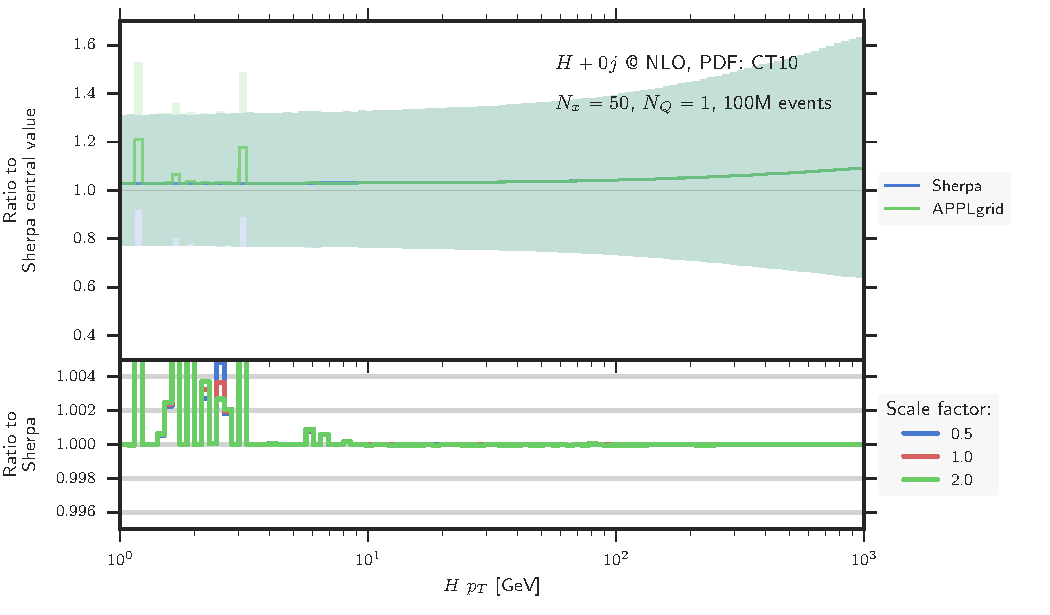
\includegraphics[width=\textwidth]{images/scalesvar_hnlo_appl.pdf}
	\caption{Scale variation appl}
	\label{fig:scalesvar_hnlo_appl}
\end{figure}
%
\begin{figure}
	\centering
	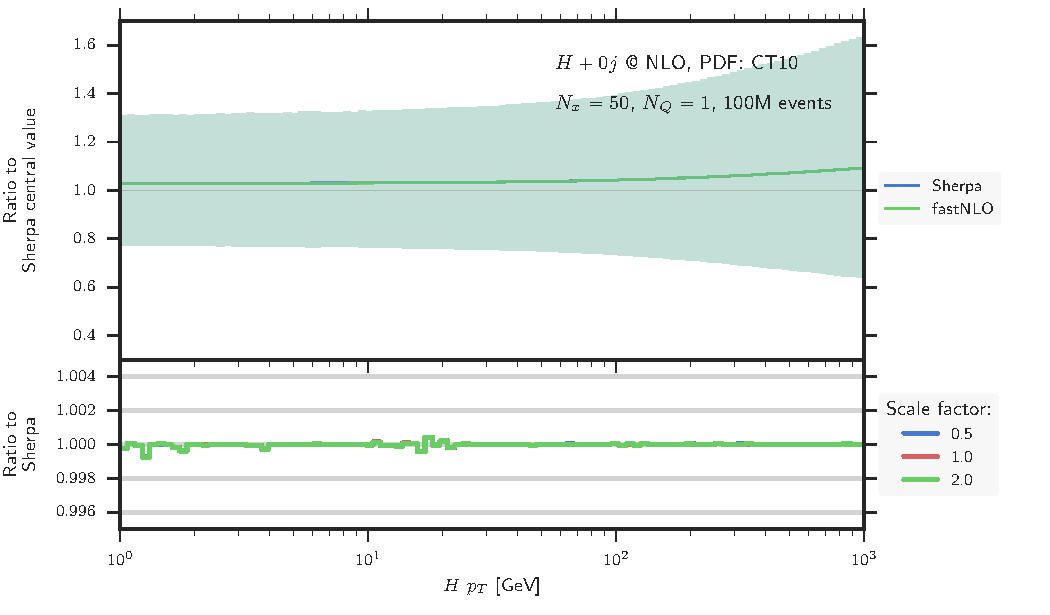
\includegraphics[width=\textwidth]{images/scalesvar_hnlo_fnlo.pdf}
	\caption{Scale variation fnlo}
	\label{fig:scalesvar_hnlo_fnlo}
\end{figure}
%
\begin{figure}
	\centering
	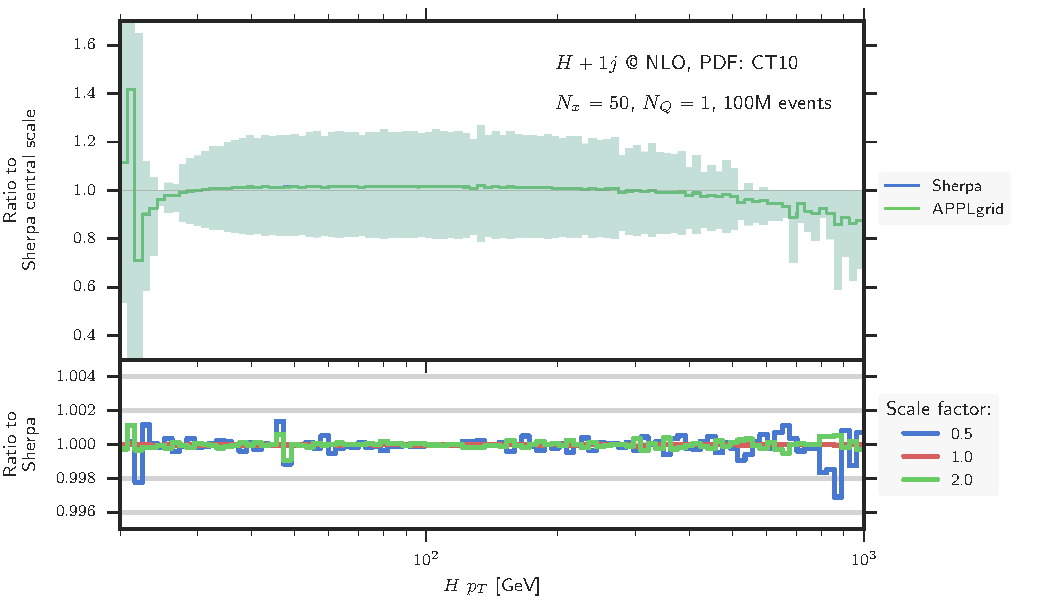
\includegraphics[width=\textwidth]{images/scalesvar_hjnlo_appl.pdf}
	\caption{Scale variation appl}
	\label{fig:scalesvar_hjnlo_appl}
\end{figure}
%
\begin{figure}
	\centering
	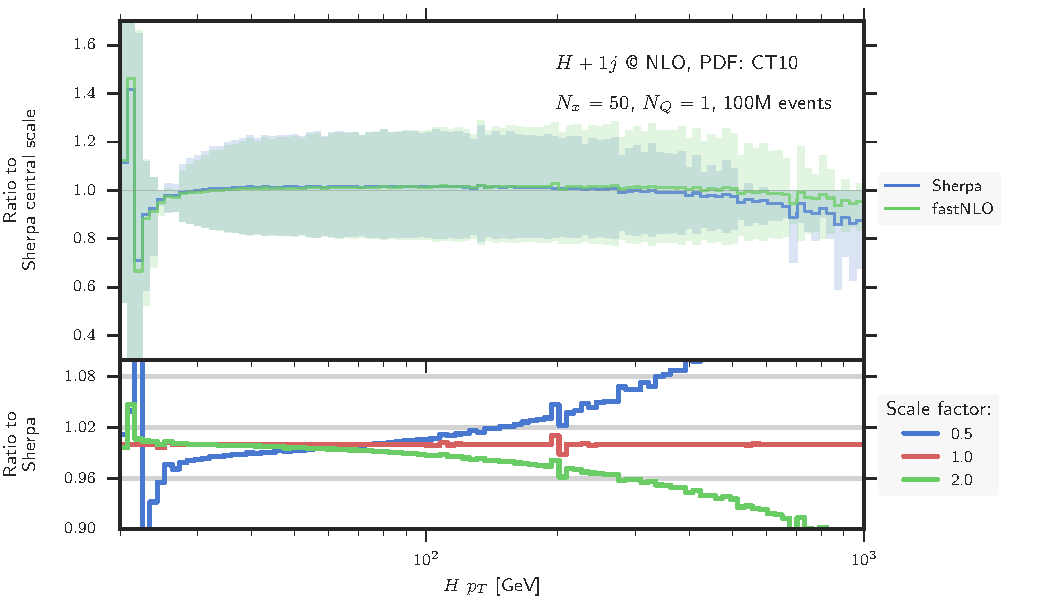
\includegraphics[width=\textwidth]{images/scalesvar_hjnlo_fnlo.pdf}
	\caption{Scale variation fnlo}
	\label{fig:scalesvar_hjnlo_fnlo}
\end{figure}
%

\section{Application example: PDF uncertainty in cross section calculations}
The application of the interpolation method is sensible every time a calculation has to be repeated plenty of times.
This situation is given, when the uncertainty from a PDF set is meant to be included in a cross section calculation.
Modern PDF sets contain a large number of different samples that can be used to derive the inherent uncertainty.
Here we consider the NNPDF 3.0 NLO set \cite{nnpdf30}, which consists of \num{101} samples each for \num{5} different values of $\alpha_s$ between \num{0.115} and \num{0.121}.
The grid that has been filled with 100 million events using the central value of the CT10 set is used to calculate a total of 505 replicas for the Higgs $p_\perp$ in \cref{fig:nnpdf_band}.
%
\begin{figure}
	\centering
	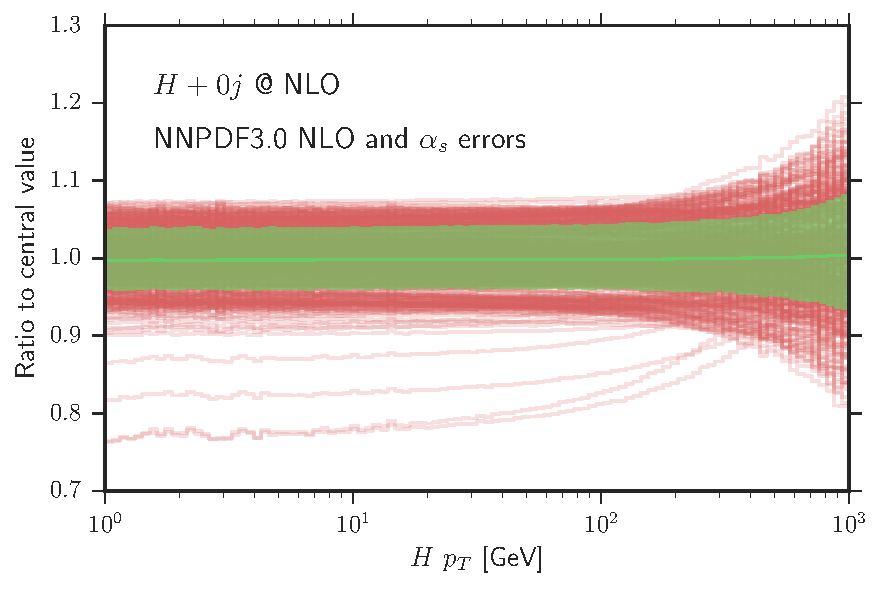
\includegraphics[width=\textwidth]{images/nnpdf_band.pdf}
	\caption{Application example of the interpolation method.
				The figure shows the distribution of replicas from the NNPDF3.0 NLO set including the error on $\alpha_s$ for the $p_\perp$ of the Higgs boson in gluon fusion.
				The green area highlights the 1-$\sigma$ confidence interval.}
	\label{fig:nnpdf_band}
\end{figure}
%
\section{Application example: Detailed scale dependence of the cross section}
When one wishes to estimate the uncertainty of a fixed order calculation, a common method is to vary the renormalization and factorization scales simultaneously or independently by some factor, usually a factor of 2.
This way one hopes to get a reasonable estimate of the corrections due to higher order terms.
Typically, only the boundary values are calculated because of limited resources.
However, using interpolation grids, any combination of scale factors can be evaluated very fast.
To demonstrate this, \cref{fig:3dscale} shows the total cross section of inclusive Higgs production through gluon fusion for different combinations of scale factors, calculated using a \fnlo{} grid.
Both the renormalization scale and the factorization scale are independently varied by 13 factors between $\frac{1}{4}$ and \num{4} resulting in a total number of 169 calculations of the cross section.

We see that the dependence on the factorization scale is low whereas we observe a strong dependence on the renormalization scale.
%
\begin{figure}
	\centering
	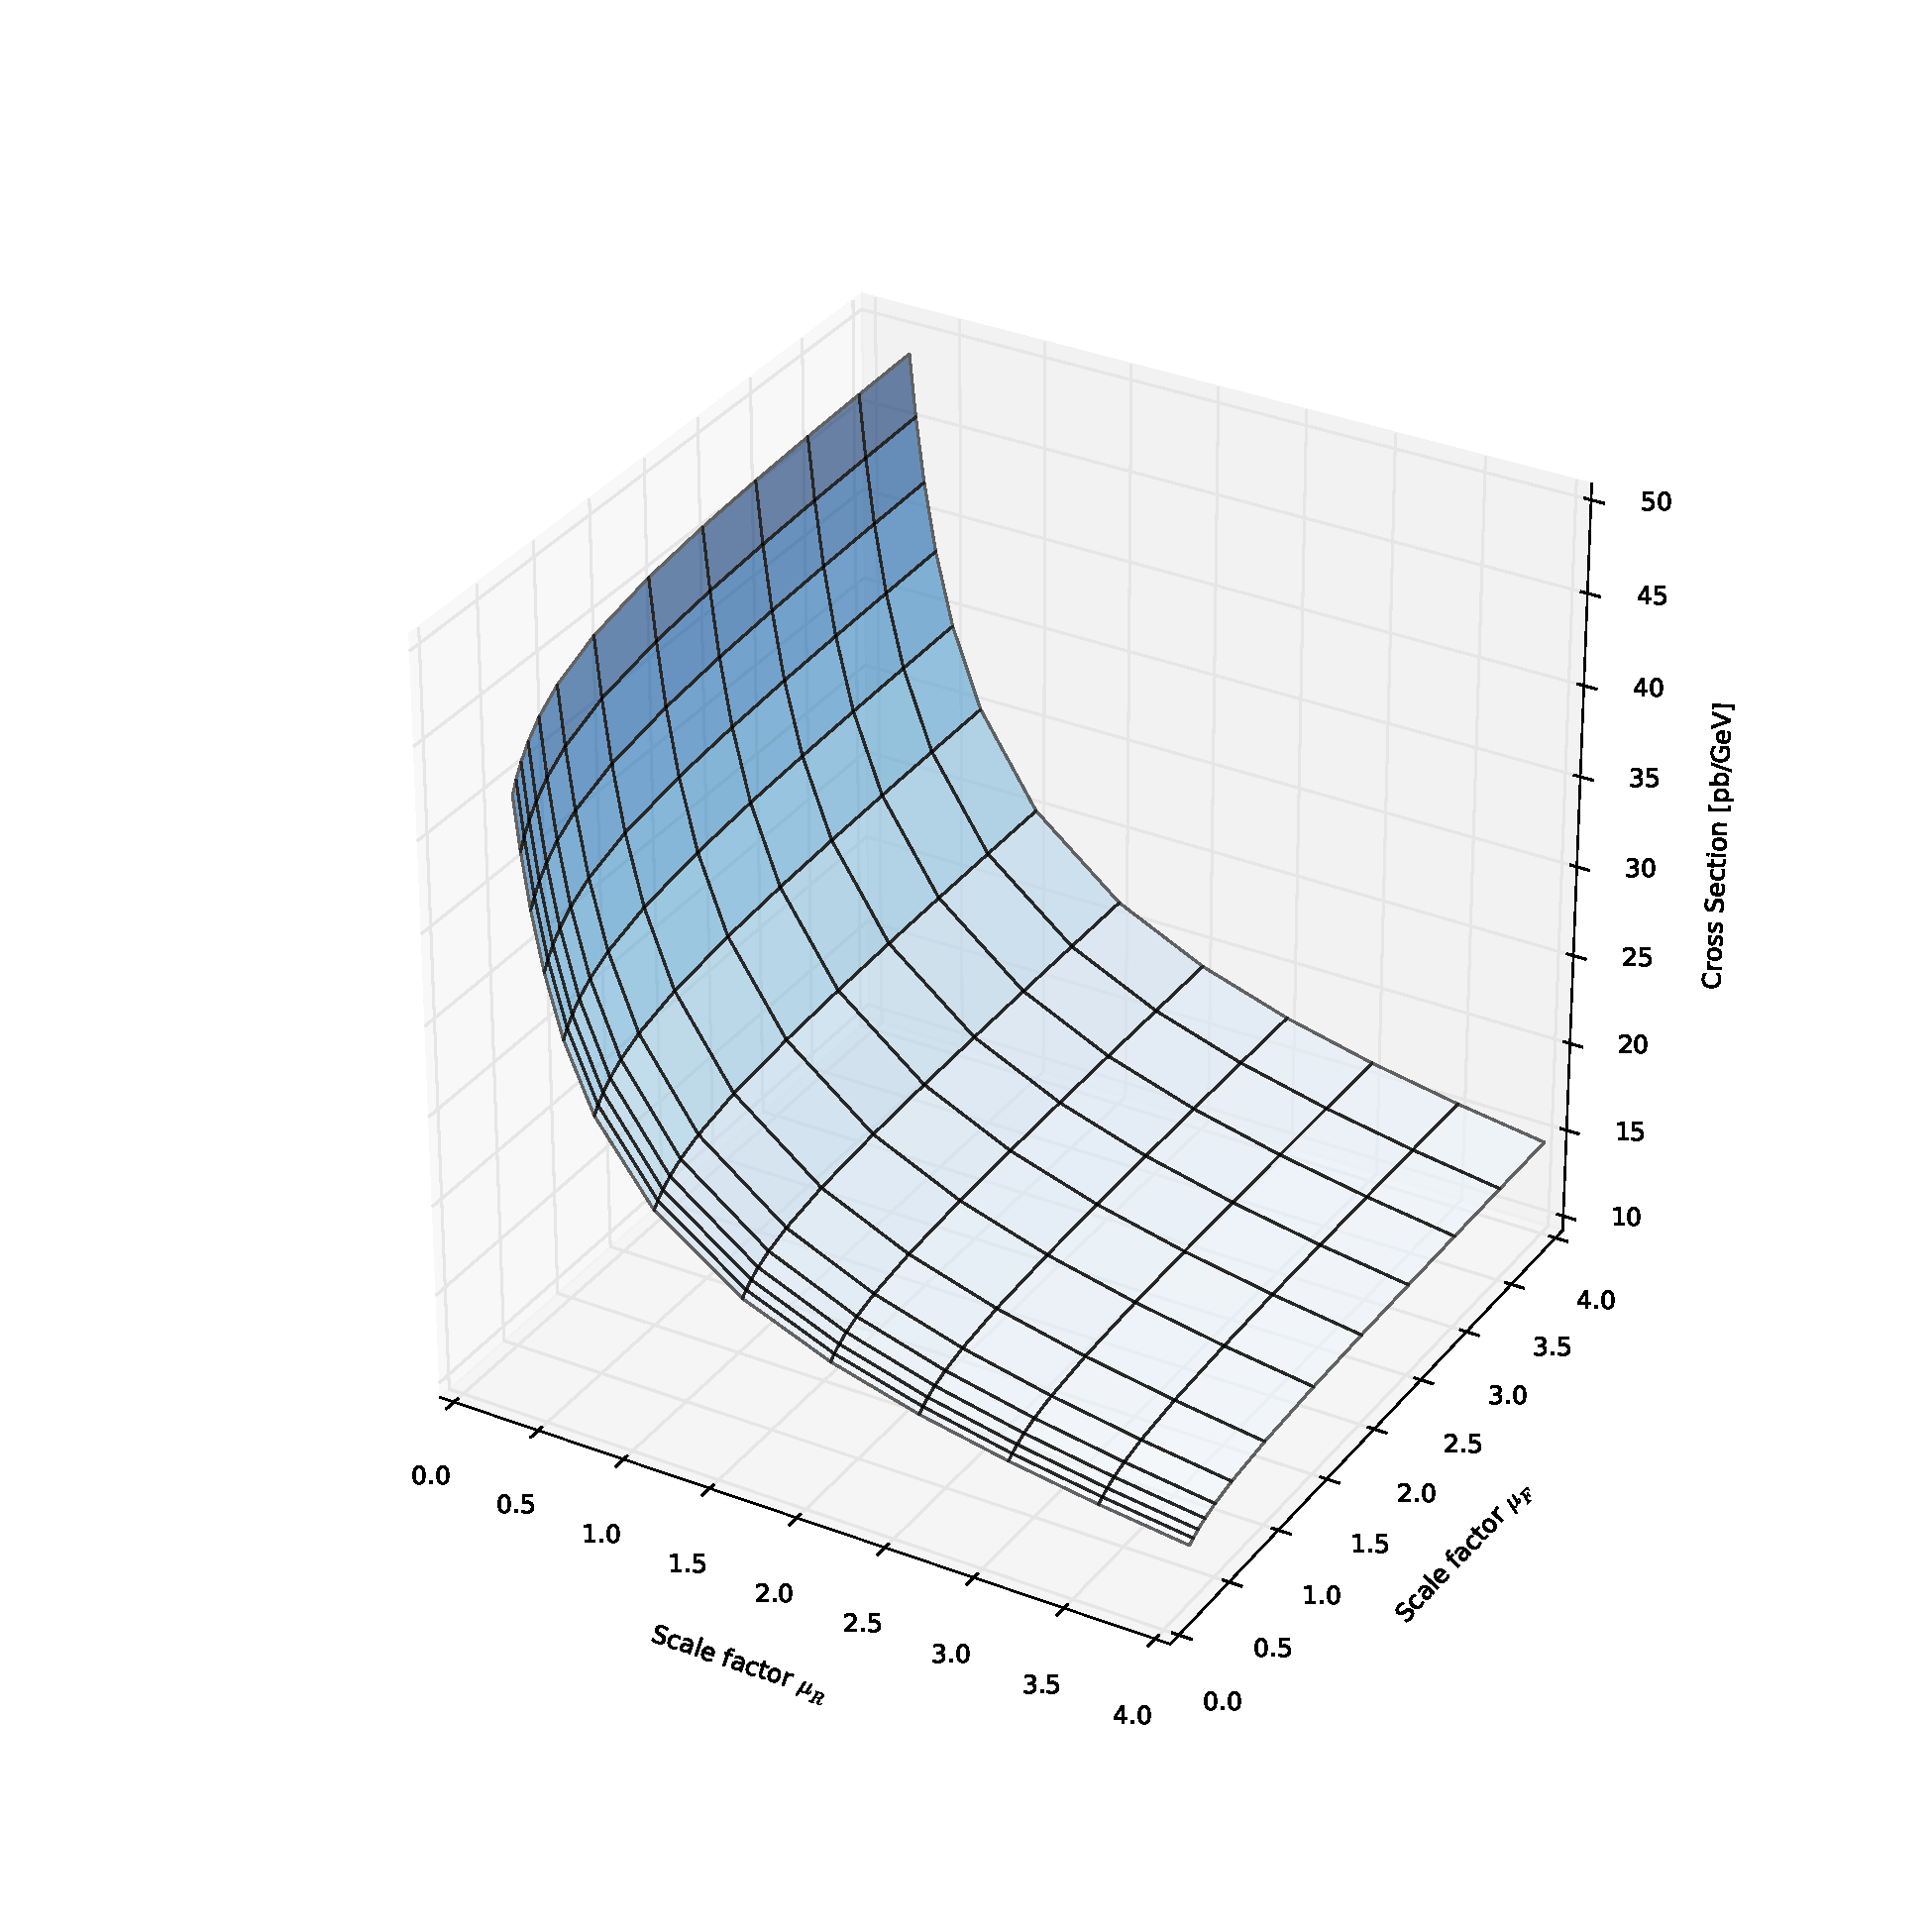
\includegraphics[width=\textwidth]{images/3dscale.pdf}
	\caption{Application example of the interpolation method}
	\label{fig:3dscale}
\end{figure}
%

Calculations such as this one and the example illustrated before would be extremely costly if done explicitly.
If they are time-critical, explicit calculations become impossible.
Interpolation tools offer much more flexibility in these cases.
